In this experiment the angular correlation and anisotropy of $\gamma$-radiation is measured.

\section{Angular distribution of $\gamma$-radiation}

When an excited state of a nucleus with spin $J_{1}$ transitions into a state with Spin $J_{2}$, the resulting distribution of $\gamma$-rays is isotropic, if the following conditions are met:
\begin{itemize}
 \item the degenerate substates of the initial state are equally occupied
 \item all permitted transitions are observed
\end{itemize}
As an example the transition between a state with $J_{1}=1$ and $J_{2}=0$ is considered. The excited state is threefold degenerate, corresponding to the three possible magnetic quantum numbers $m_{1}=1,\,0,\,-1$. The ground state is not degenerate.
The selection rule for electric dipole transitions is, that the magnetic quantum number changes by $\pm1$ or remains unchanged. Thus all three excited states can decay into the ground state. The transition probabilities are given as \cite{BB} 
\begin{align}
 W_{+} \d\Omega &= \frac{3}{16}\pi\left(1+\cos^{2}\theta\right)\d\Omega, \\
 W_{0} \d\Omega &= \frac{3}{8}\pi\sin^{2}\theta\d\Omega, \\
 W_{-} \d\Omega &= \frac{3}{16}\pi\left(1+\cos^{2}\theta\right)\d\Omega,
\end{align}
where $\d\Omega$ is an infinitesimal solid angle element and $\theta$ the angle between the direction of emission and the quantisation axis.
While the sum of all probabilities is independent of $\theta$ and therefore isotropic, the individual probabilities are not isotropic.

There are two methods of creating anisotropic $\gamma$-radiation:
\begin{itemize}
 \item Applying an external magnetic field: The application of an external magnetic field $H$ to the sample lifts the degeneracy of the initial states. Their occupation numbers change according to Boltzmann-statistics
	\begin{equation}
	 \frac{N_{i}}{N_{j}} = \exp\left(-\frac{\Delta E}{\kb T}\right),
	\end{equation}
	where $\Delta E$ is the energy difference between two levels which is given as $\mu_{\textrm{B}}H\frac{m_{i}-m_{j}}{J}$. Thus the energy levels aren't equally populated anymore and therefore the resulting radiation is in general not isotropic.
 \item Simultaneous measurement of two transitions: Now the anisotropy is created by simultaneously measuring two correlated transitions. As an example the following cascade is considered: $J_{1}=0$, $J_{2}=1$ and $J_{3}$ arbitrary. Now the first transition is characterised by the probabilities which were discussed above. For the second transition the intermediate state $J_{2}=1, \, m_{2}=0$ is not occupied and therefore the emission probailities for the second $\gamma$-quant are not isotropic.  
\end{itemize}

In the experiment the second method is used. The differential cross section for a cascade of two $\gamma$-quants with angle $\theta$ between their respective directions of emission is \cite{BB}
\begin{equation}
 \frac{\d\sigma}{\d\Omega} = \sum_{i=1}^{i_{max}} A_{2i}P_{2i}\left(\cos\theta\right), \quad i_{max}= \textrm{min}(L_{1},L_{2},J_{2}),
\end{equation}
where the $P_{2i}$ are the Legendre-Polynomials. The correlation function is given as
\begin{equation}
 K(\theta) = \frac{\d\sigma(\theta)}{\d\Omega} / \frac{\d\sigma(\SI{90}{\degree})}{\d\Omega}.
\end{equation}
This quantity is more useful in the experiment. The anisotropy can then be characterised by
\begin{equation}
 An = K(\SI{180}{\degree})-1.
\end{equation}

\section{Interaction of $\gamma$-radiation with matter}

Photons are uncharged particles. Their interaction with matter is governed by the rules of quantum electrodynamics. In matter the intensity of a $\gamma$-ray decreases, because photons are absorbed. The intensity of $\gamma$-radiation in matter is given as
\begin{equation}
 I(x) = I(0) \exp\left(-\mu x\right),
\end{equation}
where $\mu$ is the linear absorption coefficient and $x$ the traveled distance. Besides absorption, the ways $\gamma$-quants interact with matter are the following:
\begin{itemize}
 \item Compton-effect: Here a $\gamma$-quant collides with an nearly free electron from an outer shell. In this process the $\gamma$-quant loses energy. The energy which the $\gamma$ transfers to the electron is \cite{BB}
	\begin{equation}
	  \Delta E = \frac{\frac{E^{2}}{E_{0}}\left(1-\cos\theta\right)}{1+\frac{E}{E_{0}}\left(1-\cos\theta\right)},
	\end{equation}
	where $E_{0}$ is the rest energy of the electron, $E$ the energy of the incident $\gamma$-quant and $\theta$ the scattering angle. Thus there is a maximum energy transfered to the electron
	\begin{equation}
	 \Delta E_{\textrm{max}} = \frac{2E^{2}}{2E+E_{0}},
	\end{equation}
	which is always stricty smaller than $E$. Thus there is a maximum energy up to which compton-scattered $\gamma$-quants are detected. This is known as the compton-edge. In the experiment only unscattered $\gamma$-quants ought to be detected. Therefore only events with an energy of about $60$-$70\%$ of the expected energy are counted.
 \item Photoeffect: Here a $\gamma$ knocks a bound electron out of an atom and is absorbed by the atom. The kinetic energy of the released electron is related to the energy of the $\gamma$-quant.
 \item Pair creation: If a $\gamma$ possesses an energy greater than two times the electrons mass $E\geq2m_{e}c^{2}\approx\SI{1}{\mega\electronvolt}$, pair creation can occur. In this process the $\gamma$ annihilates into an electron-positron-pair. The process occurs only in the vicinity of a heavy nucleus, since momentum has to be conserved.
\end{itemize}


\section{Experimental realisation}

In the experiment the $\beta^{-}$-decay from $^{60}$Co to $^{60}$Ni (see figure \ref{fig:term}) is used. $^{60}$Ni transitions into the ground state while emitting a cascade of two $\gamma$-rays ($L_{1}=2,\,L_{2}=2$: electric quadrupole radiation). The intermediate state has spin $J_{2}=2$. Thus it holds
\begin{equation}
 K(\theta) = 1 + a_{2}\cos^{2}(\theta) + a_{4}\cos^{4}(\theta),
\end{equation}
with $a_{2}=\frac{1}{8}$ and $a_{4}=\frac{1}{24}$. \cite{BB}

\begin{figure}[tb]
 \centering
 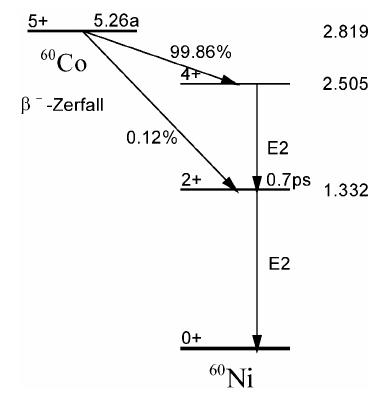
\includegraphics[scale=0.8]{./fig/termschema.png}
 \caption{Term diagram of the transition from $^{60}$Co to $^{60}$Ni \cite{BB}}
 \label{fig:term}
\end{figure}

For the measurement two NaI-scintillators are used. One of them can be placed in angles $\SI{180}{\degree},\,\SI{135}{\degree},$ and $\SI{90}{\degree}$ relative to the other. To get only the $\gamma$-rays from the cascade, a coincidence-measurement is used. Nevertheless, random coincidences may be counted as well. The rate between the number of true coincidences $N_{c}$ and the number of random ones $N_{r}$ is approximately given as
\begin{equation}
 \frac{N_{c}}{N_{r}} \approx \frac{1}{\tau_{\textrm{A}}A},
\end{equation}
where $\tau_{\textrm{A}}$ is the resolving time of the detector and $A$ the activity of the sample.



